%%%%%%%%%%%%%%%%%%%%%%% file typeinst.tex %%%%%%%%%%%%%%%%%%%%%%%%%%%%%%
%
% This is the LaTeX source for the instructions to authors using
% the LaTeX document class SVMultln with class option 'lnicst'
% for contributions to the Lecture Notes of the Institute for
% Computer Sciences, Social-Informatics and
% Telecommunications Engineering series.
% www.springer.com/series/XXXX       Springer Heidelberg 2007/08/05
%
% It may be used as a template for your own input - copy it
% to a new file with a new name and use it as the basis for
% your article. It contains a few tweaked sections to demonstrate
% features of the package, though.
%
% If you have not much experiences with Springer LaTeX support,
% you should better use the special demonstration file "lnicst.tex"
% included in the LaTeX package for LNICST as template.
%
%%%%%%%%%%%%%%%%%%%%%%%%%%%%%%%%%%%%%%%%%%%%%%%%%%%%%%%%%%%%%%%%%%%%%%%%

\documentclass[lnicst,sechang,a4paper]{svmultln}
\usepackage{amssymb}
\setcounter{tocdepth}{3}
\usepackage{graphicx}

\usepackage{url}
\urldef{\mailsa}\path|{mohsin.khan, valtteri.niemi}@helsinki.fi|
\usepackage[pdfpagelabels,hypertexnames=false,breaklinks=true,bookmarksopen=true,bookmarksopenlevel=2]{hyperref}


%added by the author himself
\usepackage{color}
\usepackage[numbers]{natbib}
\usepackage{calc}
\usepackage{siunitx}
\DeclareSIUnit\mt{\milli\tesla} %% A method for say short cut or new unit!
\sisetup{inter-unit-product = {-}}

\begin{document}

\mainmatter  % start of an individual contribution

% first the title is needed
\title{Privacy Protected Subscriber Identification in 5G Network}
%Concealing IMSI in 5G Network Using Identity Based Cryptography

% a short form should be given in case it is too long for the running head
\titlerunning{Concealing IMSI in 5G Network Using Identity Based Cryptography}

% the name(s) of the author(s) follow(s) next
%
% NB: Chinese authors should write their first names(s) in front of
% their surnames. This ensures that the names appear correctly in
% the running heads and the author index.
%
\author{Mohsin Khan%
%%\thanks{Please note that the LNICST Editorial assumes that all authors have used
%%the western naming convention, with given names preceding surnames. This determines
%%the structure of the names in the running heads and the author index.}%
\and Valtteri Niemi}  %
%\authorrunning{Lecture Notes of ICST: Authors' Instructions}
% (feature abused for this document to repeat the title also on left hand pages)

% the affiliations are given next
\institute{University of Helsinki, Department of Computer Science,\\
P.O. Box 68 (Gustaf H\"allstr\"amin katu 2b)\\
FI-00014 University of Helsinki\\
Finland\\
\mailsa
%\\
%\url{http://www.springer.com/series/7911}
}

%
% NB: a more complex sample for affiliations and the mapping to the
% corresponding authors can be found in the file "lnicst.dem",
% that is contained in the LNICST LaTeX support package.
%

\toctitle{AES and SNOW 3G are Feasible Choices}
\tocauthor{Authors' Instructions}
\maketitle


\begin{abstract}
The aspirations for the next generation mobile network (5G) are high. It has a vision of improved security and privacy over the existing LTE network. Subscription privacy of a user has been a historical concern with all the previous generation mobile networks, namely GSM, UMTS, and LTE. While a little improvement have been achieved in securing the privacy of long-term identity of a subscriber, the so called IMSI catchers are still in existence even in the LTE and advanced LTE networks. This report looks into this problem of concealing long-term identity of a subscriber and presents different techniques of using public-key cryptography to tackle it. One special case of public-key crytography is identity based crypto. A rigorous comparison among the pros and cons of the different techniques show that identity based cryptograpy is a potential solution for securing the long-term identity privacy of a user in the 5G network.
\end{abstract}


\section{Introduction}
\label{intro} NGMN Alliance has pointed out the privacy of a user as a requirement of the 5G network under the requirement category of enhanced services \cite{NGMN_white_paper}. In 3GPP TR 33.899 \cite{TR33899}, subscribers' privacy is captured as one of the high level security requirements of the 5G network. However, in the context of diversified devices and the complex business and service model of 5G, it is important to define who is a subscriber and what subscriber-privacy means. According to 3GPP TR 21.905 \cite{TR21905} a subscriber is an entity (associated with one or more users) that is engaged in a subscription with a service provider. A subscription describes the commercial relationship between the subscriber and the service provider, cf. 3GPP TR 21.905 \cite{TR21905}. A subscription identifier is the identifier that uniquely identifies a subscription in the 3GPP system. The identifier is used to access networks based on 3GPP specifications. Subscription Privacy refers to the right to the protection to any information that (a) can be used to identify a subscription to whom such information relates, or (b) is or might be directly or indirectly linked to a subscription. This definition of privacy suggests to protect any personally identifiable information (PII) from an active or passive attacker. While it is important to classify the identifiers into PII and non-PII, the long-term identifier is surely a PII. In this report we will keep our discussion limited only to the case of identification of an UE using long-term identifier of the relevant subscriber. In the case of 2G (GSM), 3G (UMTS) and 4G (LTE) networks, this long-term identifier is known as international mobile subscriber identity (IMSI). Nevertheless, the same principles used in the solutions proposed in this report can be extended to conceal any PII.


One approach of protecting IMSI privacy is to use a temporary IMSI instead of the original IMSI and keep changing the temporary IMSI at a feasible frequency. Note that the temporary IMSI has to be assigned over a confidentiality protected channel and different entities of the network may assign different temporary IMSIs to the user equipment (UE). In the LTE network, the temporary IMSI assigned by serving network (SN) is called globally unique temporary identity (GUTI) and the home network (HN) does not assign any temporary IMSI to the UE. However, during the initial attachment of a UE to the SN, the UE has neither a GUTI nor a security context with the SN that can assign it with a GUTI. Besides, GUTI can be lost by either one or both of the UE and the SN. This forces the UE to reveal its IMSI to the SN to keep itself from permanently locked out of the network. This problem gives an opportunity to an active IMSI catcher (AICa) who impersonates a legitimate SN and forces the UE to run the initial attachment protocol. This also gives an opportunity to a passive IMSI catcher (PICa) to eavesdrop the IMSI sent in clear text. Solutions \cite{pseudonym_valtteri_philip, pseudonym_ericsson} have been proposed by using temporary IMSI known as pseudonym assigned by the HN. While these solutions solve the cases of lost and unsynchronised GUTI, they still have the problem of lost or unsynchronised pseudonyms and also initial attachment. In this report we present how a security context can be set up in between the network (either with SN or HN) and the UE even before the identification of the UE so that the UE can use the security context to send its IMSI with confidentiality protection. Such a security context will mitigate the attack mounted by a PICa. Nevertheless, we show that an AICa would not be able to agree on a legitimate security context with the UE and consequently will not be able to reveal the IMSI.

\begin{figure}
\begin{center}
% Use the relevant command to insert your figure file.
% For example, with the graphicx package use
  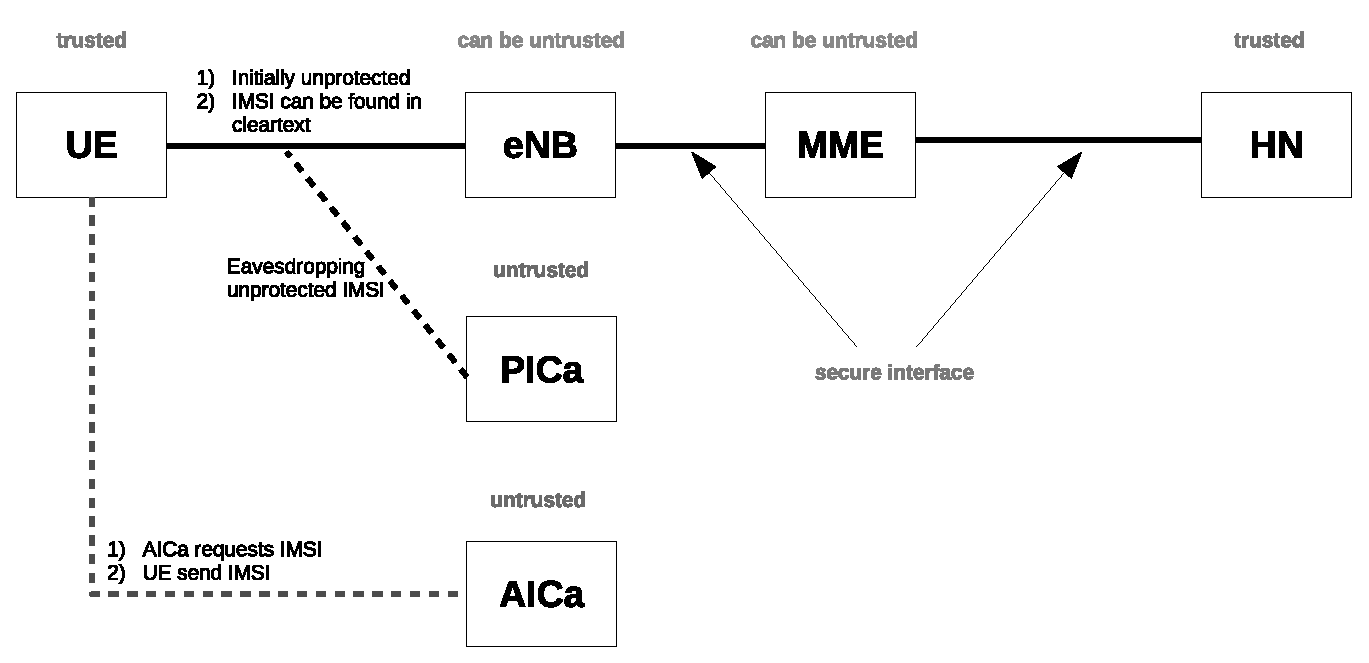
\includegraphics[width=.98\textwidth]{security_architecture_abstraction.eps}
% figure caption is below the figure
\caption{High-level security architecture}
\label{fig:security_architecture_abstraction}       % Give a unique label
\end{center}
\end{figure}

In order to present a formal discussion we need to know what are the entities involved in this identification process, what are the communication interfaces among those entities and how much the entities can be trusted with the IMSI.  As the architecture of 5G security is yet to be finalized, we present an abstraction of the involved entities and assume that whatever the security architecture of 5G eventually be, it will contain these entities and interfaces. This abstraction is directly extracted from LTE security architecture. Figure \ref{fig:security_architecture_abstraction} shows the entities. It involves the UE, serving radio network (SRN), serving core network (SCN), HN. We have two more entities: PICa and AICa. The interface  UE-NB in between UE and SRN is initially unprotected. Nevertheless, SRN-SCN and SCN-HN are always protected and the security of these interfaces is out of the scope of this report. The PICas eavesdrop on the UE-SRN interface when it is unprotected to extract an IMSI. The AICas impersonate a legitimate SN and run a legitimate protocol with the UE in order to reveal the IMSI. HN and UE both own the IMSI and they are trusted with it. Both of PICa and AICa are untrusted while it is technically possible to not trust SRN and SCN. However, by some other specification in 3GPP TS \textcolor{red}{xx.xxx} it is required to reveal IMSI to the SCN to enable lawful interception (LI) without involving HN. 

We propose different solutions based on public-key cryptography which make the UE-SRN interface protected even during the initial attachment to fight against the PICa. Our solutions also stop the AICa from running a legitimate protocol successfully that could reveal the IMSI. However, there are other 5G requirements which our solutions should also meet. Such requirements are: reduced signalling overhead, improved control plane latency, concealing all the parts of IMSI (MCC, MNC and MSIN). To avoid the downgrade attack, the solutions need to be backward compatible with the legacy networks. Also, in the case of public-key, the complexity involved in setting a PKI and revocation of a publick-key need to be considered with high importance. Considering all these requirements, we evaluate our solutions based on the following criteria:
\begin{enumerate}
\item Concealed from PICa, AICa, SRN, SCN
\item Parts of the IMSI concealed
\item Signalling overhead
\item Latency
\item Backward compatibility
\item PKI complexity
\item Public-key revocation and re-provisioning 
\end{enumerate}
While the choice of the solution is dependent on how much want to achieve, hybrid solution using identity based public-key cryptography and pseudonyms appear to be a promising solution.

In Section \ref{sec:id_based_crypto} we present a quick intro to identity based cryptography (IBC). In Section \ref{sec:solutions} we present the solutions. In Section \ref{sec:evaluation}, we present a rigorous solution based on the aforementioned evaluation criteria. Finally we conclude the paper in Section \ref{sec:conclusion}

\section{IBC in the Jargon of Cryptography} \label{sec:id_based_crypto}
Modern-day cryptography can be broadly categorized into two categories depending on how the keys are used to encrypt and decrypt the message. In symmetric key cryptography the sender and receiver share a secret key which is used for encryption and decryption both. In public-key cryptography the receiver has a pair of keys. One of the keys is public and the other is private. The public key is used by the sender to encrypt the message and the private key is used by the receiver to decrypt the message. While the challenge in symmetric key cryptography is to create a key known only by the sender and receiver but no one else, one major challenge in public-key cryptography is to authenticate the public key.

\begin{figure}
\begin{center}
% Use the relevant command to insert your figure file.
% For example, with the graphicx package use
  \includegraphics[width=.98\textwidth]{ibc_in_jargon_of_crypto.eps}
% figure caption is below the figure
\caption{IBC in the Jargon of Cryptography}
\label{fig:ibc_in_the_jargon_of_cryptography}       % Give a unique label
\end{center}
\end{figure}

Based on the authentication mechanism, public-key cryptography can be categorized into three more categories:
\begin{enumerate}
\item Certificate based
\item Root-key based
\item Identity based, which is known as IBC
\end{enumerate} Figure \ref{fig:ibc_in_the_jargon_of_cryptography} shows this categorization with advantages and disadvantages of the respective categories. In the certificate based case, the public key is signed by a trusted third party. In the root-key based case, no runtime authentication of the public key is required because a very limited number of public key is used in the system and all the senders are pre-provisioned with all the existing public keys. In the IBC case, the public key of a receiver is computed from the identity of the receiver and the public key of a trusted third party. However, the private key of the receiver is computed from the identity of the receiver and the private key of the trusted third party. This private key has to be securely provisioned to the receiver by the trusted third party. In this case, even though an extra one-time burden of private key provisioning is required, the sender does not need to authenticate the public key of a receiver, because if the public key is not authentic, the receiver will not have the private key and any message encrypted by the public key will never be decrypted. In other words, the authenticity of the public key in IBC is guranteed by the trusted third party. Usually in IBC, the trusted third party is known as the private key generator (PKG). While in the certificate based and root-key based case it is possible to revoke the public key of a receiver, it is impossible to revoke the public key in IBC unless the identity itself is revoked. In Figure \ref{fig:how_ibc_works} we show how IBC works pictorially.


\begin{figure}
\begin{center}
% Use the relevant command to insert your figure file.
% For example, with the graphicx package use
  \includegraphics[width=.98\textwidth]{how_ibc_works.eps}
% figure caption is below the figure
\caption{IBC mechanism}
\label{fig:how_ibc_works}       % Give a unique label
\end{center}
\end{figure}

\section{Solutions}\label{sec:solutions} 
\label{sec:solutions}
It would be beneficial to mention some notation here before delving into the solutions. 
\begin{enumerate}
\item $hnid=MCC||MNC$ identifies the HN
\item $scnid=MCC||MNC$ identifies the SCN
\item $e_A$ is the public key of entity $A$
\item $d_A$ is the private key of entity $A$ 
\item $\mathcal{X}_{A,B}$ is the certificate of the public key of $A$ issued and signed by $B$
\item $E,D$ are the encryption and decryption functions respectively
\end{enumerate}


\subsection{Certificate Based Public-key Cryptography} 
\label{sub_sec:solution_certificate}
In certificate based public-key cryptography, certificates digitally signed by a trusted third party is used to authenticate the ownership of a public key. The trusted third party who can sign the certificate is called a certificate authority (CA). It is possible to build a chain of trust in certificate based public-key cryptography by allowing an entity to become a CA who is certified by a CA. A certificate contains a digital signature which allows anyone to verify the validity of the certificate by verifying the digital signature using the public key of the CA who provided the certificate. There has to exist at least one CA in a chain of trust whom the verifier already trusts. There might exist entities who certifies itself and some verifiers trust these entities. The entities having a self signed certificate who are trusted by verifiers is considered as the root CA for those verifiers and the corresponding certificates are called root certificates. To use certificate based public-key cryptography to secure IMSI privacy, we need to figure out few things first: who are the root CAs and who else can be a CA, who are the entities that own a public key, how a certificate can be revoked and how the UE can be re-provisioned with a new root certificate if required.

We choose the HN of a subscriber as the root CA for the subscriber. HN owns a self signed certificate which is the root certificate. Every UE having a subcription of the HN is provisioned with the root certificate. An SCN owns a public key certified by HNs. The SRN broadcasts the SCN's identity. The UE interested to attach with the SCN sends its $hnid$ to the SRN and SRN relays it to SCN. SCN sends its public key certificate provided by the HN of the UE. SRN relays the certificate to the UE. The UE verify the certifiate. If it is a valid signature, the UE concatenates some random bits called $salt$ at the end of the IMSI, encrypts the result with the public key of SCN and sends the ciphertext to the SRN. The SRN relays this to the SCN. SCN decrypts the ciphertext, discard the salt from the tail and extracts the IMSI. This completes the identification of a UE to SCN. Figure \ref{fig:solution_certificate} shows the protocol in detail. Note that, in the roaming agreement phase, the SCN does not need to get the certificate exactly from the HN but can get it from any CA who is trusted in by the HN the chain of trust.


\begin{figure}
\begin{center}
% Use the relevant command to insert your figure file.
% For example, with the graphicx package use
  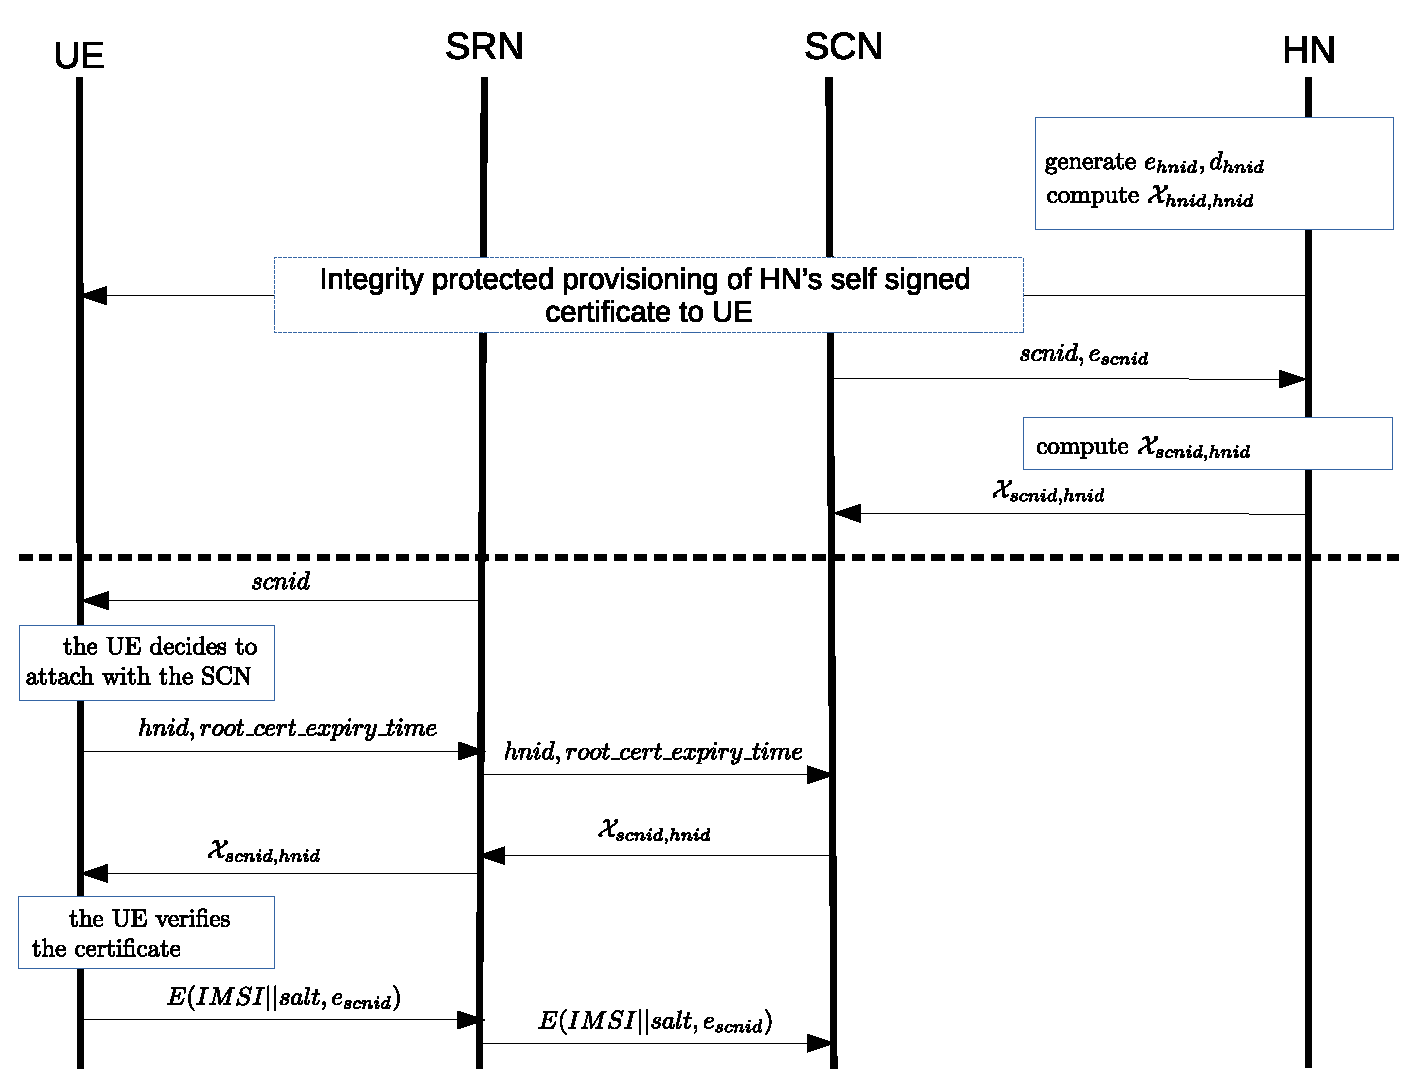
\includegraphics[width=.98\textwidth]{public_key_variation1.eps}
% figure caption is below the figure
\caption{Privacy protected UE identification using certificate based public-key cryptography}
\label{fig:solution_certificate}       % Give a unique label
\end{center}
\end{figure}

This approach can not conceal MCC and MNC at all. It coneals MSIN from AICa, PICa and SRN. The IMSI is revealed entirely at SNC. It requires a full round trip signalling in betwenn UE and SCN before sending the encrypted MSIN. It carries $hnid$ from UE to SCN and in return carries the public-key certificate back from SCN to UE. Public keys are quite large, length of a minimum ciphertext is also very long comparatively, and the certificate chain can be quite long. Consequently it adds signficant signalling overhead. Also, public-key cryptography is computationally heavier than that of symmetric-key cryptography. As a result, latency will increase significantly to verify the certificate and encrypt the IMSI Nevertheless, once an UE is identified by the network, the network assigns a GUTI to the UE. It is a question for further research to evaluate the effect of this extra signalling overhead and increased latency. This solution is not backward compatible with LTE, UMTS and GSM. It doesn't require to establish any new trusted authority, so PKI complexity is very little. However, revocation of the public-key of an SCN and HN is not trivial and need to be investigated closely.

Every CA in the system maintains a list of revoked public keys which were certified (at the first place) by it or by any other CA trusted by it. If there is a revocation, the CA who provided the certificate at the first place updates its revoked list and the CA updates its CA with the information. The UE periodically runs a protocol with HN to download the latest revoked public keys. If a dishonest SCN presents an UE with the certificate which is already revoked but the UE has not yet been able to downloaded it, then the MSIN will be revealed to the SCN. However, such a dishonest SCN will fail to run a successful authentication protocol. As soon as the UE come in touch with a legitimate SCN, it identifies itself successfully, runs a successful authentication protocol, and download the latest revocation list from the HN. Thereafter the dishonest HN will not be able to reveal the MSIN any more. This implies that an AICa can mount an attack if it was once trusted by the HN as a legitimate SCN but is no more trusted by the HN and the UE is not yet updated with the withdrawal of the trust. The existence of such an AICa is apparently extremely rare. The time window this attack allows to track a subscriber is also very small. Altogether this makes the attack very expensive. However, if the private key of an SCN is stolen, both PICa and AICa can mount attacks until the public key is revoked. 

When the private key of an HN is compromised, the HN updates itself with a new public-private key pair and generate a new root certificate. All the relevant certificates in the system get updated with the required changes according to the standard PKI procedure. However, every UE that has a subscription with the HN needs to be re-provisioned with the new root certificate. Because, if an SCN is updated with the new certificate, but the UE does not have the new root certificate, then the UE will never be able to verify the certificate presented by a legitimate SCN. To circumvent this problem the SCN stores certificates chained with all the root certificates used by an HN. The SCN first checks the $root\_cert\_timestamp$ sent by the UE. The SCN then finds the certificate provided by the HN in which the root certificate has the same time stamp as $root\_cert\_timestamp$. Consequently, an SCN whose certificate is not chained with the latest root certificate of an HN, will not be able to reveal the MSIN of an UE. Once the UE is identified by the SCN and authentication becomes successful, the HN knows the location of the UE. At this point the HN can send the new root certificate to the UE integrity protected by the master symmetric key shared by the HN and the USIM. Another way is to publish the new root certificate in the public media with integrity protection so that anyone can download the root certificate using some other internet connection. The need for re-provisioning the UE with a new root certificate is an extremely rare event. In case the root private key is stolen by an attacker, it allows the attacker to act as both AICa or PICa. Once the need for existing root certificate revocation and provisioning of a new one is identified, it does not allow the attacker a long time window to track the UEs. However, protecting the privacy of a private key and detecting the compromise of a private key is a whole different security question and we do not delve into that in this report.


\subsection{Solution based on a Single Root-key} 
\label{sub_sec:solution_root-key}

This is called root-key based solution because there is only one public key that an UE needs to know about. It is the public key of the HN and we call it to be the root-key. This public key is provisioned to all the UE which have subscriptions with the HN. Whenever an UE is in need of identifying itself to a SCN with the IMSI, the UE encrypts the IMSI with the public root key and sends the result to the SCN along with the $hnid$. Note that the UE concatenates a random salt at the end of the IMSI before encryption to avoid having the same encryption result every time. The SCN sends the encrypted IMSI to the appropriate HN. The HN decrypts and extracts the IMSI. To facilitate LI, the HN sends back IMSI to SCN with both integrity and confidentiality protection.Figure \ref{fig:solution_root-key1} shows the protocol in detail.


\begin{figure}
\begin{center}
% Use the relevant command to insert your figure file.
% For example, with the graphicx package use
  \includegraphics[width=.98\textwidth]{root-key1.eps}
% figure caption is below the figure
\caption{Privacy protected UE identification using a single root-key}
\label{fig:solution_root-key1}       % Give a unique label
\end{center}
\end{figure}



This approach can not conceal MCC and MNC at all. It conceals MSIN from AICa, PICa, SRN and SCN. It doesn't need to transfer and verify the certificate each time the protocol is run. It reduces the signalling and computational overhead than that of certificate based solution. However, the problem of heavier computation for public-key encryption and large ciphertext expansion remains as downsides of this solution.  Nevertheless, once an UE is identified by the network, the network assigns a GUTI to the UE. It is a question for further research to evaluate the effect of these downsides in signalling overhead and increased latency. This solution is not backward compatible with LTE, UMTS and GSM. It doesn't require to establish any new trusted authority, so there is no PKI complexity involved.

When the private key of the HN is compromised, the HN generates a new pair of keys. All the UEs of the HN has to be re-provisioned with the new public key. If not, then someone who has access to the private key will be able to eavesdrop the encrypted IMSI and decrypt it. Also someone who gets access to the private key will be able to mount an active attack. However, if the public key in the HN is changed and an UE not provisioned with the new public key sends the encrypted IMSI to the HN via a legitimate SCN, the HN will not be able to decrypt it with the new private key. To circumvent this problem, the HN provides a key identifier while provisioning an UE with a public key. And the UE sends the key identifier ($kid$) along with the encrypted IMSI to inform the HN which private key should be used decrypt the IMSI. 


\subsection{Solution based on IBC} 
\label{sub_sec:solution_ibc}


\begin{figure}
\begin{center}
% Use the relevant command to insert your figure file.
% For example, with the graphicx package use
  \includegraphics[width=.98\textwidth]{solution_based_on_ibc.eps}
% figure caption is below the figure
\caption{Privacy protected UE identification using IBC}
\label{fig:solution_ibc}       % Give a unique label
\end{center}
\end{figure}


%Here we use public key cryptography which may or may not be based on identity based crypto to secure the privacy of the long term identity of a mobile phone user called IMSI (International mobile subscriber identity). We discuss different techniques of using the public key cryptography:

%\begin{enumerate}
%\item Identity based crypto based on the identity of SN where the HN is the key generator
%\item HN assigned public private key pair for each SN
%\item HN owned public private key pair
%\end{enumerate}

%In the consequent sections we describe the aforementioned techniques in further detail.

%\section{Based on Identity of Serving Network} In this technique the HN has a public and private key pair. Every phone knows the public key of the HN. Whenever a SN asks the phone to provide its IMSI, the phone computes the public key of the SN using the public key of the HN. Then the phone encrypts the IMSI with the computed public key of the SN and sends it to the SN along with the HN identity. The SN obtains (possibly already have obtained) its private key from the mentioned HN. Using this private key, the SN can decrypt IMSI. Figure \ref{fig:IBC} represents the high level protocol.

%\subsection{Concerns and Solutions}
%\begin{enumerate}
%\item How to provision, revoke and re-provision the public key of HN in the phone?
%\item How to black list a SN?
%\end{enumerate}

%\subsection{Based on HN generated public private key pair for every SN}

\section{Conclusion}
\label{sec:conclusion}

\section{Acknowledgement}
\label{sec:acknowledgement}



\begin{thebibliography}{4}

\bibitem{NGMN_white_paper} NGMN 5G White Paper V1.0 [cited Jan, 2017]. Available at: https://www.ngmn.org/uploads/media/NGMN\_5G\_White\_Paper\_V1\_0.pdf

\bibitem{TR33899} 3GPP TR 33.899 V0.6.0 [cited Jan, 2017]. Available at: https://portal.3gpp.org/desktopmodules/Specifications/SpecificationDetails.aspx?\\specificationId=3045

\bibitem{TR21905} 3GPP TR 21.905 [cited Jan, 2017]. Available at: https://portal.3gpp.org/desktopmodules/Specifications/SpecificationDetails.aspx?\\specificationId=558


\bibitem{pseudonym_ericsson} Karl Norrman, Mats Näslund, Elena Dubrova: Protecting IMSI and User Privacy in 5G Networks. 2nd International Workshop on 5G Security

\bibitem{pseudonym_valtteri_philip} Philip Ginzboorg,  Valtteri Niemi: Privacy of the long-term identities in cellular networks. Proceedings of the 9th EAI International Conference on Mobile Multimedia Communications
Pages 167-175




\end{thebibliography}

\end{document}
